\documentclass{article}
\usepackage[a4paper, total={5.2in, 9in}]{geometry}
\usepackage{graphicx} % Required for inserting images
\usepackage{parskip}
\usepackage{listings}
\usepackage{xcolor}
\usepackage{amsmath}
\usepackage{amssymb}
\usepackage{mathtools}
\usepackage{caption}
\usepackage{subcaption}
\lstset{
tabsize = 4, %% set tab space width
showstringspaces = false, %% prevent space marking in strings, string is defined as the text that is generally printed directly to the console
numbers = left, %% display line numbers on the left
commentstyle = \color{green}, %% set comment color
keywordstyle = \color{blue}, %% set keyword color
stringstyle = \color{red}, %% set string color
rulecolor = \color{black}, %% set frame color to avoid being affected by text color
basicstyle = \small \ttfamily , %% set listing font and size
breaklines = true, %% enable line breaking
numberstyle = \tiny,
}

\newcommand{\paren}[1]{\left(#1\right)}

\title{ACS Programming Assignment 3}
\author{Rikke Tophøj Heinemann (DTZ190) \\ Marie Elkjær Rødsgaard (DCK495) \\ Rasmus Pallisgaard (DWP992)}
\date{January 4. 2024}

\begin{document}

\maketitle

\section{Discuss in detail the setup you have created for your experiments}

In this assignment we experiment with how our book store service handles multiple client and manager requests at the same time. All experiments were run on a machine with a 6-core Intel Core i7 (9750H) with a 12MB shared cache across all cores. The machine has 16GB of DRAM and runs MacOS 14.2.1 (Sonoma). For each experiment the book store was initialized with 10 different books, each with an ISBN $i$ between 1 and 10, along with the names 'bookTitle $i$' and authors 'author $i$'. Initially each book store is given $100$ copies of each book in order to ensure that we do not encounter too many failed interactions as a result of a lack of copies of a book. Each book was given a price of 10, and all books were set to be editor picks. All other book parameters were given default values of 0.

The initial setup above then encounters 3 different types of interactions from a differing number of clients. The interactions are:
\begin{enumerate}
	\item A frequent interaction by clients of the book store was to find pick 10 random editor picked books, then purchase 1 copy of 5 of them. 60\% of interactions constituted this type. The number of copies bought was chosen since it practice is rare for somebody to buy multiple copies of the same book, and the number of books considered was chosen to balance the fact that the book store initially only stored 10 books.
	\item A frequent interaction by stock managers was to select the 5 books with the smallest quantity in stock and replenish that stock by adding 10 copies. 30\% of actions were of this type. These were chosen to balance out the outgoing book copies from the aforementioned interaction.
	\item A rare interaction by stock managers was to pick 5 random books from an external list, and add the books the books to the book store that were not present. These books were picked from an extended list of books generated using the method used for the initial state, but extended to include 100 books. Furthermore, for books with $10 < \text{isbn world} \leq 100$, the book was chosen to be an editors pick if the isbn was even. This extended list allows us to continuously add new books to the store, and include new editor picks to vary the other interactions. This interaction was chosen 10\% of the time.
\end{enumerate}
The format of the books added to the store initially and throughout experimentation was chosen to focus on different ISBNs rather than author and name values, since identification and handling of books in the store is based on ISBNs. Regarding the experimentation runs, we fix the value of warmup runs and experiment runs for each user that queries to the book store to $100$ and $2000$ respectively. The warmup was chosen to warm the system up, and the experiment run number was chosen to minimize noise over each experiment run, since we initially experienced great variation with lower numbers of experiment runs. During experiments we vary the number of concurrent users accessing the store, with each user following the setup above. We make this fix/variation setup in order to specifically examine how the system handles changes in concurrent accessing users, and varying the number of actions each could have unforeseen effects on experimentation.

Through experimentation we measure the aggregated throughput and average latency of the system as the number of concurrent users vary. The aggregate throughput is measured by
\begin{equation}
	\text{throughput}_\text{agg}=\sum_{\text{experiments}}\frac{\text{\# successful interactions}}{\text{experiment runtime in seconds}}
\end{equation}
And is measured in interactions per second. The average latency is measured by
\begin{equation}
	\text{latency}_\text{mean}=\frac{\sum_{\text{experiments}}\paren{\frac{\text{experiment runtime in milliseconds}}{\text{\# successful interactions}}}}{\text{\# experiment runs}}
\end{equation}
and is measured milliseconds per interaction. We choose the aggregated throughput to measure how much \underline{simultaneous} throughput the service can handle, and average latency to show the \underline{expected latency} for each user. The choices of seconds vs milliseconds comes down to which is easier to interpret for the given case ($0.014$s of latency vs $44$ms of latency).

We experiment with the following number of simultaneous users: [1, 2, 5, 10, 20, 50, 100, 200, 500, 1000, 2000]. This is to understand the metrics at drastically different scales of concurrent interaction. Creating more than 4000 concurrent threads accessing the server would crash the java process due to a lack of memory available. Each of these users' actions will be executed in different threads, with one thread per user. For each number of users we repeat the experiment 5 times and compute the average and standard deviation for each number of concurrent users to give intuition on the expected throughput/latency and deviations from it.

Our experiments will be made in two versions: First we conduct experiments across the same address space, meaning on the same machine without network interaction, and the second series of experiments are conducted across http using RPC over localhost, incurring a new cost of having to perform network requests during interactions. 

For both experiments we expect that as we increase the number of actors interacting with the book store the throughput will increase to a certain point, and latency will increase steadily. We expect the experiments across address spaces to perform generally worse than over one machine due to the overhead of performing requests and responses.

\section{Show and explain the plots for throughput and latency that you obtained.}

Figure \ref{fig:throughput-latency} shows plots obtained from our experimentation. In figure \ref{fig:throughput-all} and \ref{fig:throughput-diff} we see that as the number of thread increase, throughput increases as well up to a certain point, after which it plateaus. For the same address space this plateauing happens at around 500 concurrent actors, and across address spaces this happens at around 20 concurrent users. Furthermore we see that the aggregated throughput for each address space differs by orders of magnitude, with throughput for the same address space peaking at 25000 successful interactions/s, while only being around 450 across address spaces. This plateauing of throughput is due to the book store having a maximum throughput that the machine is able to execute for the given service, regardless of address space. The large difference in throughputs is largely due to the overhead of introducing requests and responses over network. We did expect there to be a maximum throughput but did not expect the large difference in maximum throughput the versions were able to achieve.

In figures \ref{fig:latency_all} and \ref{fig:latency-same} we see that latency increases as we increase the number of clients. Notice that since the x-axis is logarithmic, this increase is in fact linear as we increase the number of agents acting on the service. In the same address space our implementation achieved a max latency of 40ms per successful interactions, while it was a whopping 2.5 seconds per successful interactions across spaces.
We again see a large difference in values depending on if we experiment in the same address space or across address spaces, this time opposite to what we saw before. We did expect the latency to increase as we increased the number of concurrent actors. We did not expect the large differences between experiments, nor the scale of latency reached by experimenting across address spaces. 


\begin{figure}
	\centering
	\begin{subfigure}[b]{0.48\textwidth}
		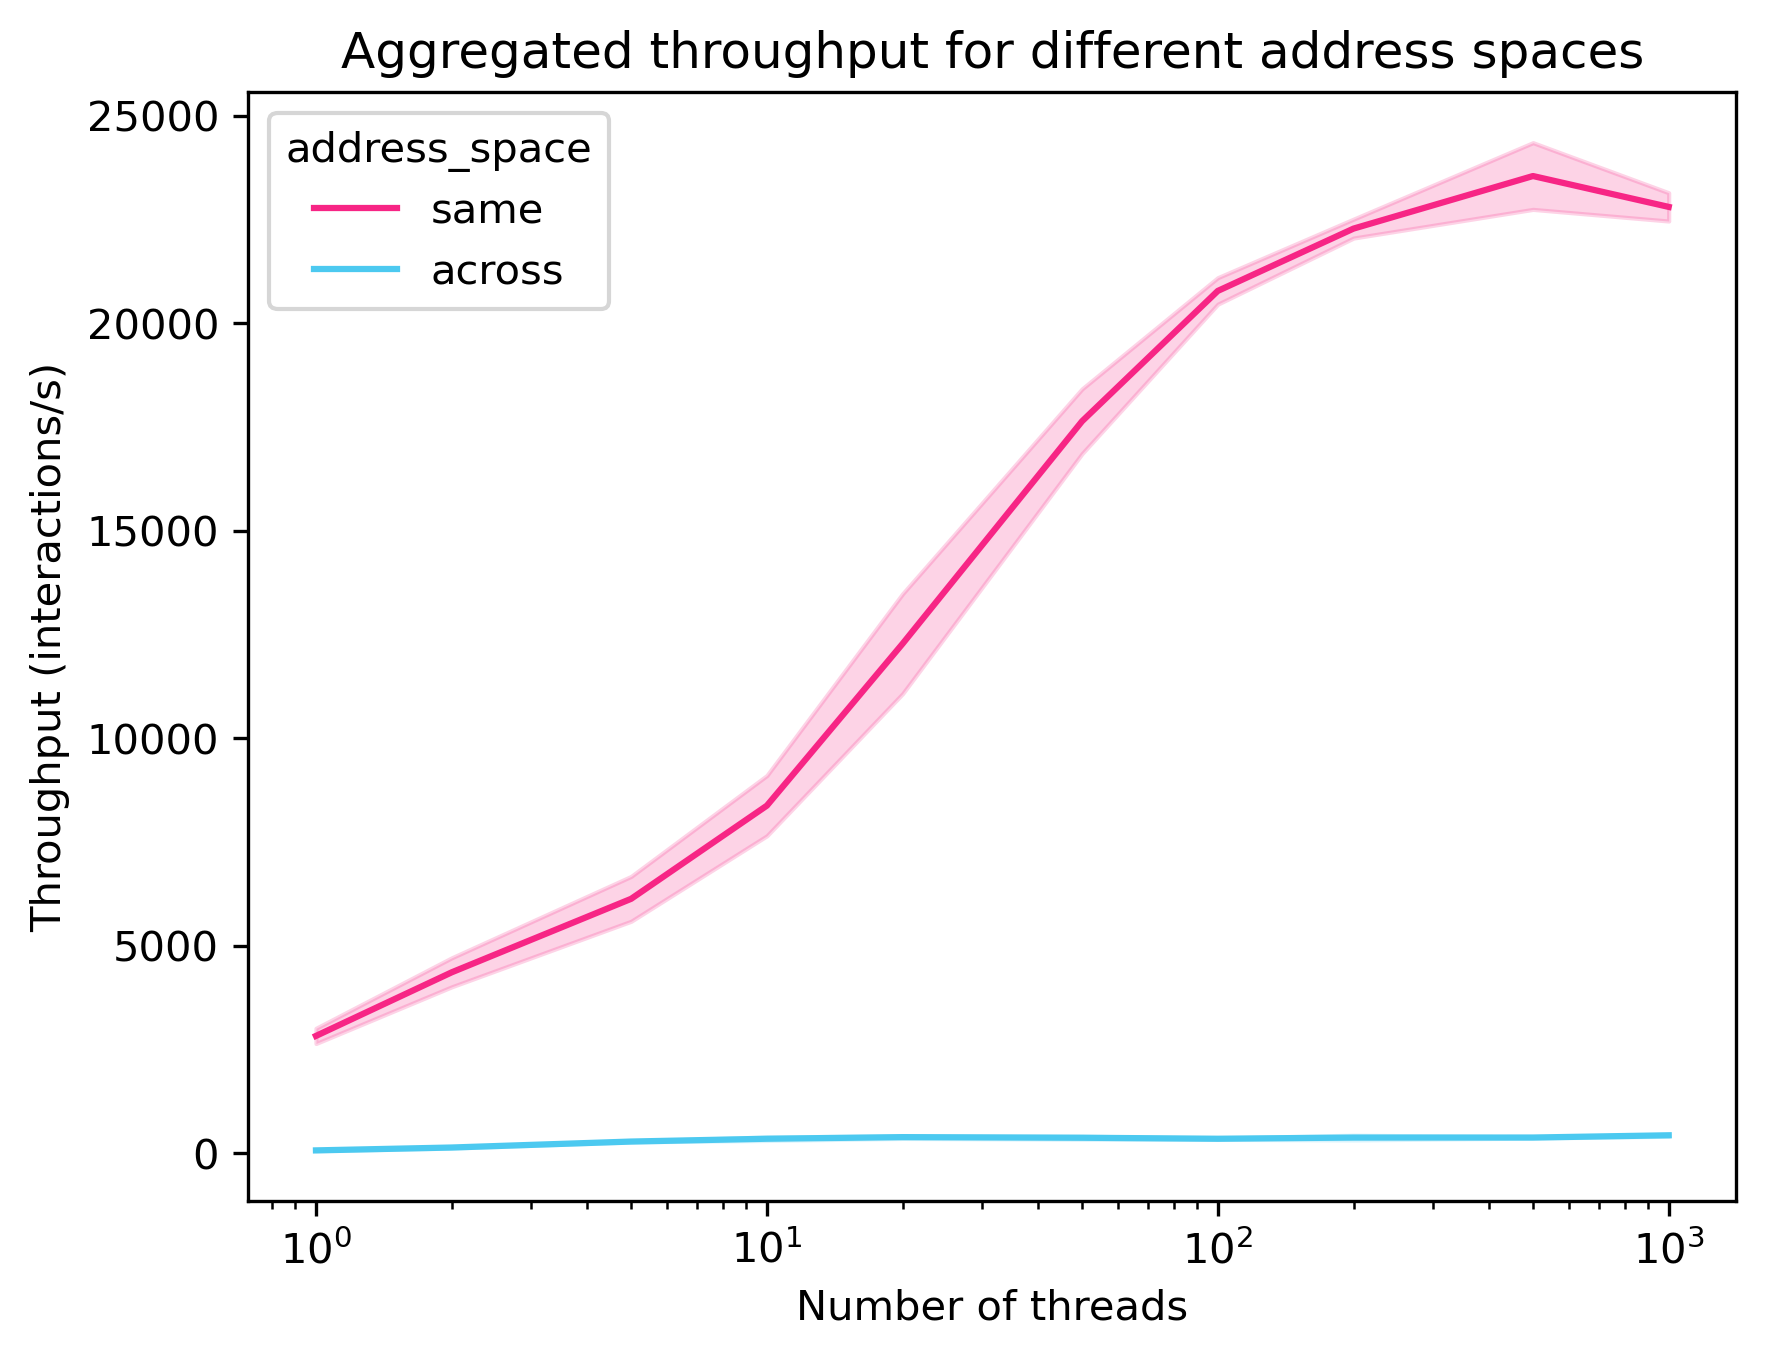
\includegraphics[width=\textwidth]{plots/throughput_all}
		\caption{Aggregated throughput for the two address spaces.}
		\label{fig:throughput-all}
	\end{subfigure}
	\hfill
		\begin{subfigure}[b]{0.48\textwidth}
		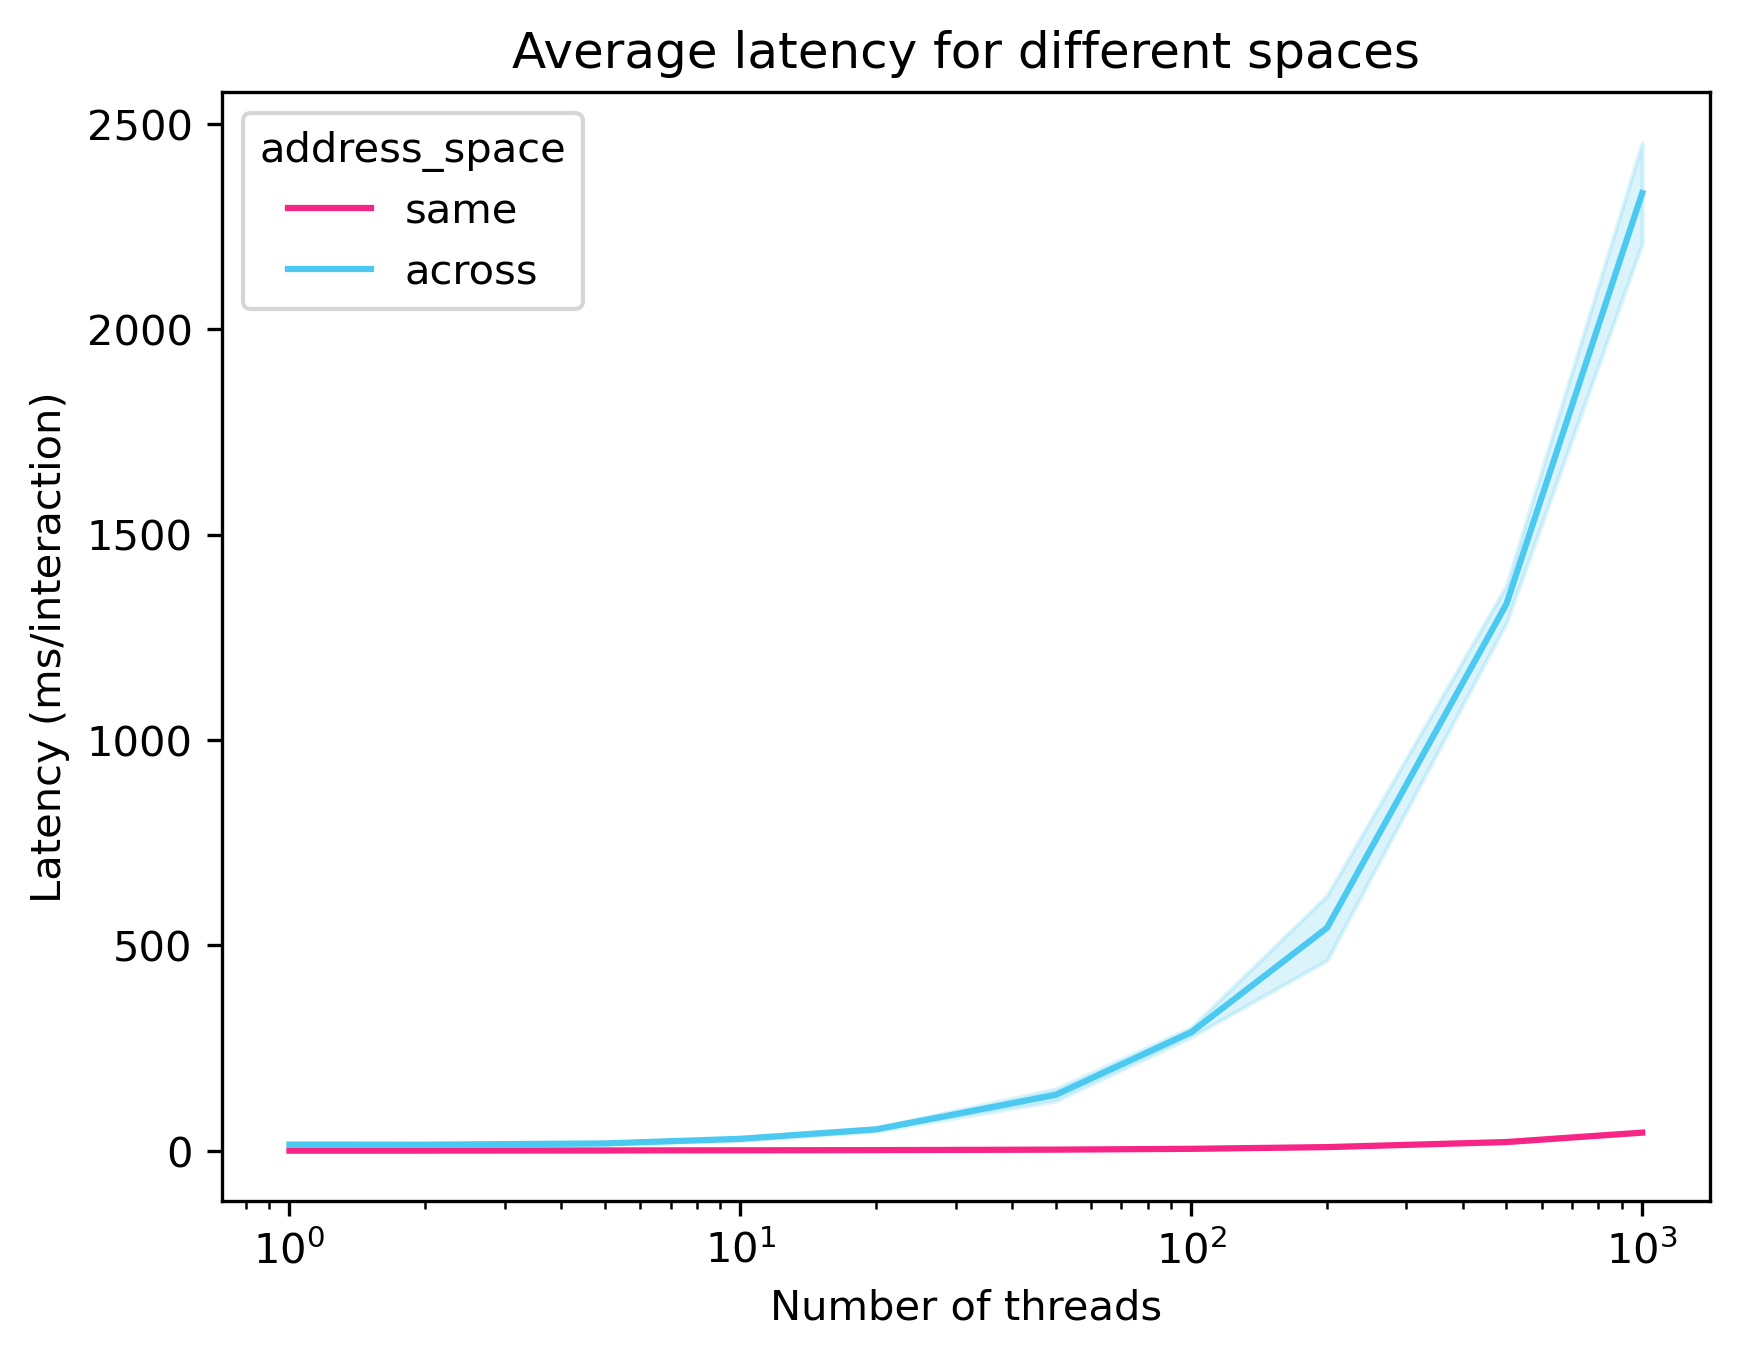
\includegraphics[width=\textwidth]{plots/latency_all}
		\caption{Average throughput for the two address spaces.}
		\label{fig:latency_all}
	\end{subfigure}
	\begin{subfigure}[b]{0.48\textwidth}
		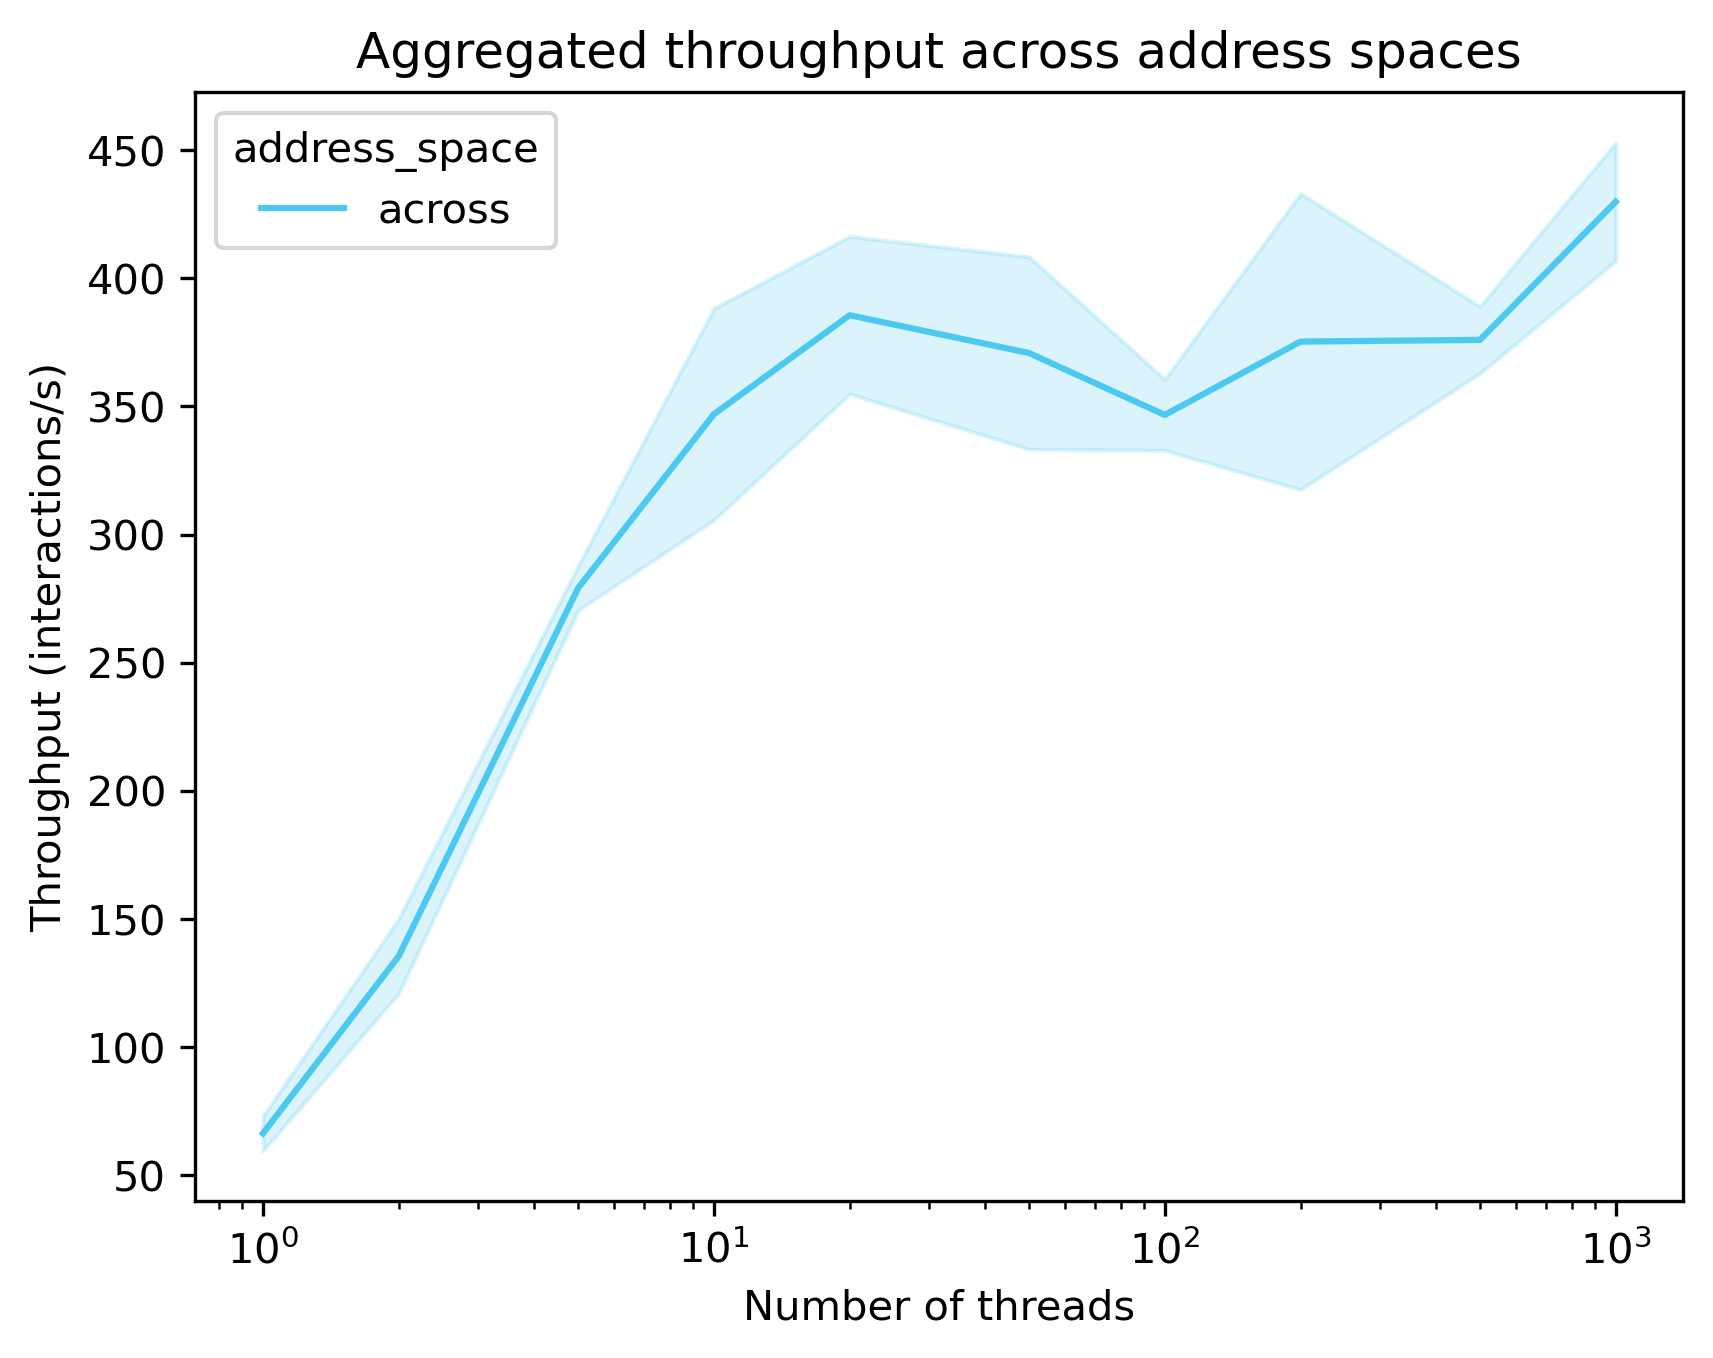
\includegraphics[width=\textwidth]{plots/throughput_diff}
		\caption{Aggregated throughput across address spaces only.}
		\label{fig:throughput-diff}
	\end{subfigure}
	\hfill
	\begin{subfigure}[b]{0.48\textwidth}
		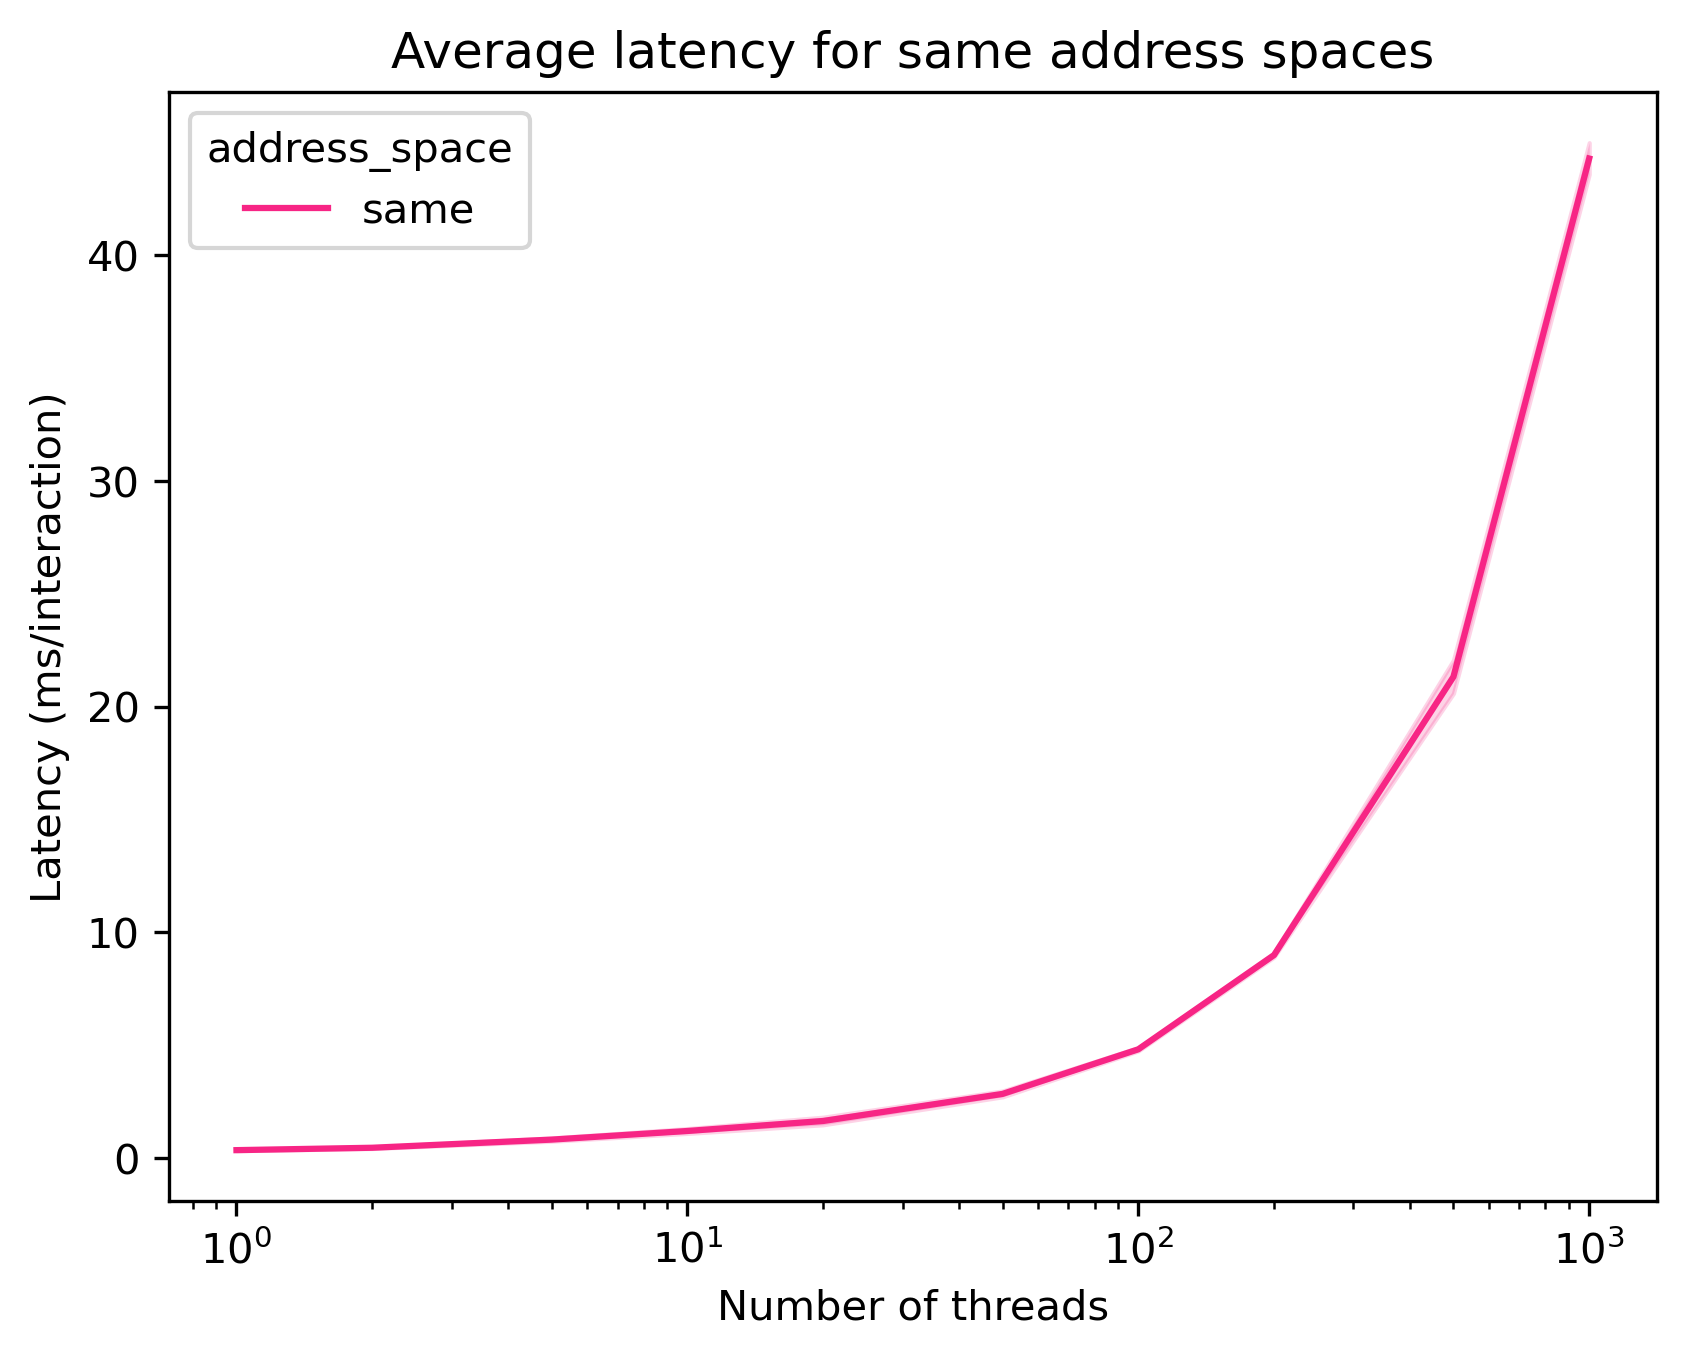
\includegraphics[width=\textwidth]{plots/latency_same}
		\caption{Average latency for the same address space only.}
		\label{fig:latency-same}
	\end{subfigure}
	\caption{Aggregated throughput and average latency measured during experimentation. Measures taken both on a local machine and over HTTP using RPC. Plots \ref{fig:throughput-diff} and \ref{fig:throughput-diff} shows a zoomed in version of throughput only across address spaces and latency only for the same address space.}
	\label{fig:throughput-latency}
\end{figure}

Finally, in order to ensure that our experiments were conducted properly we've included plots of the share of successful interactions being frequent customer interactions and the success rate over the number of threads. In figure \ref{fig:inter-and-succrate} we see that these values stayed relatively fixed at the expected $0.6$ and $\approx1.0$ respectively.

\begin{figure}
	\centering
	\begin{subfigure}[b]{0.48\textwidth}
		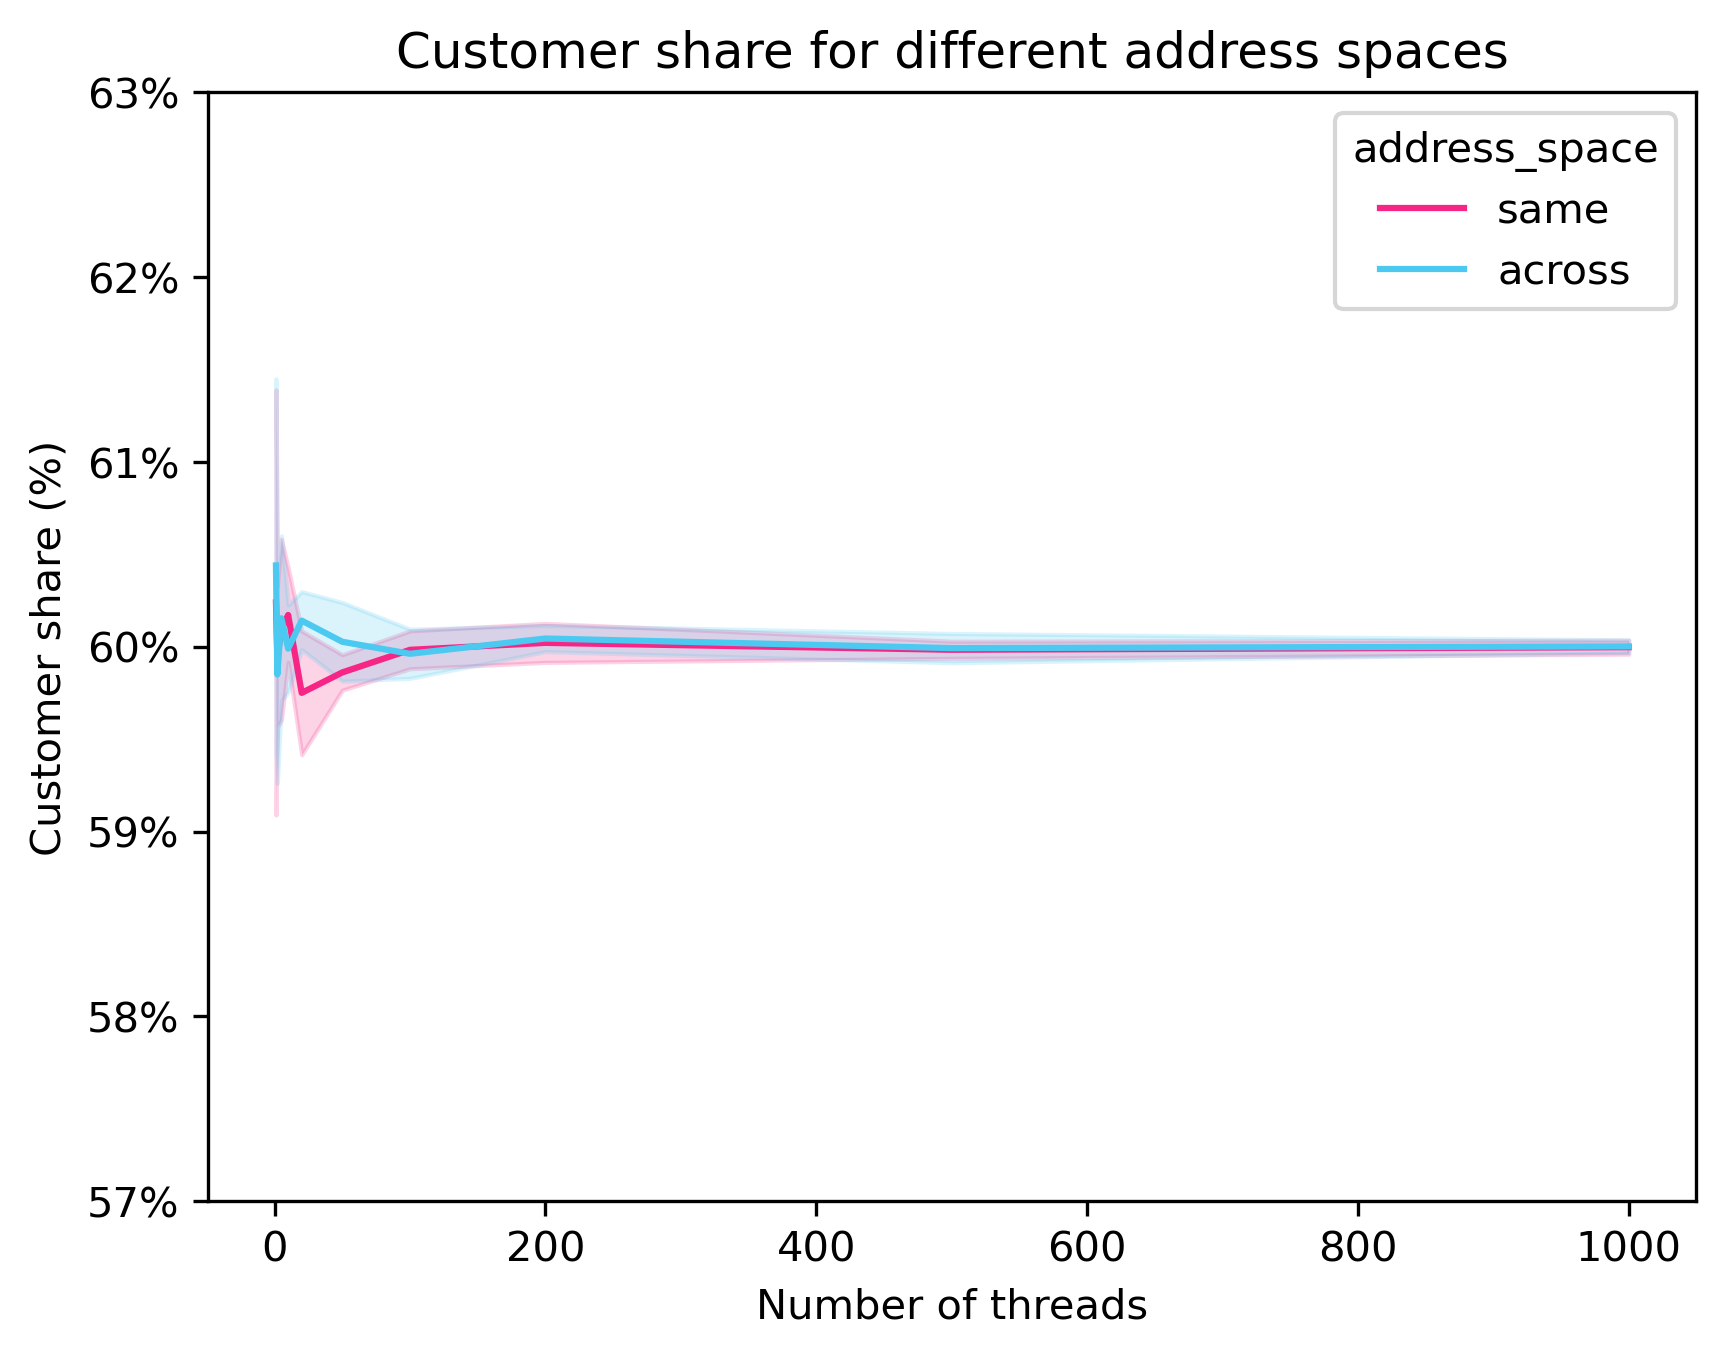
\includegraphics[width=\textwidth]{plots/customer_share}
		\caption{Share of interactions being frequent customer interactions over number of threads.}
	\end{subfigure}
	\hfill
	\begin{subfigure}[b]{0.48\textwidth}
		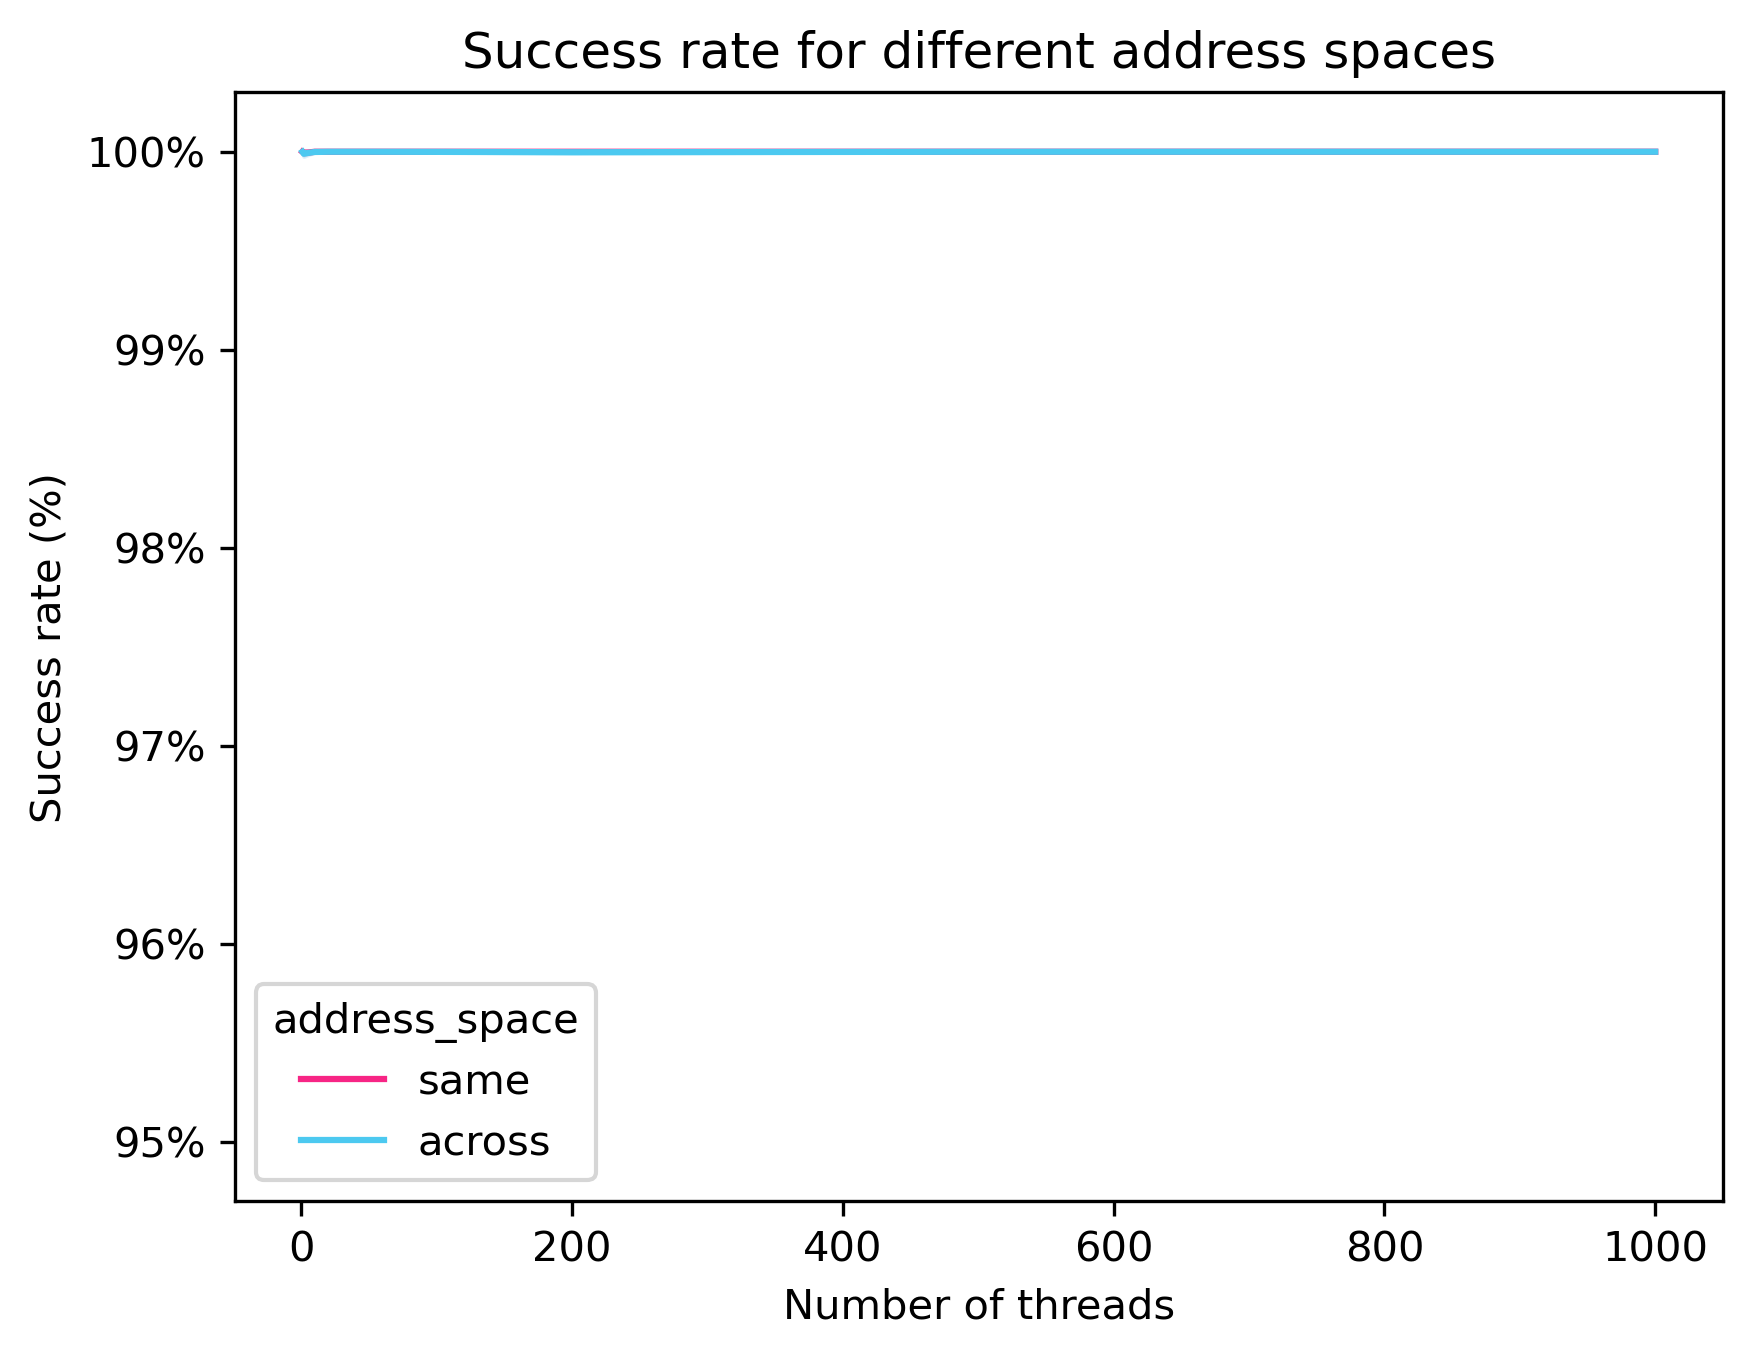
\includegraphics[width=\textwidth]{plots/success_rate}
		\caption{Success rate for our interactions over the number of threads used in our experiments.}
	\end{subfigure}	
	\caption{Plots for statistics related to experimentation.}
	\label{fig:inter-and-succrate}
\end{figure}

\section{How reliable are the metrics and the workloads for predicting the performance of the bookstore? Are the metrics well chosen? What additional metrics would you choose to demonstrate the performance of the bookstore?}

The metrics of aggregate throughput and average latency are reliable for predicting the performance: aggregated throughput relates to how much we throughput we can expect the service to handle when considering all connected clients, while average latency shows the expected latency for each user. This lets us predict performance of the system both in terms of what the book store is capable of, and in terms of what the interaction will be like for the user. The workload is theoretical and might not immediately reflect reality, as it for example isn't often that one user repeatedly buys one copy of 5 books 2000 times. However, is reliable in the sense that this repeating of workloads helps produce reliable results on average, as extreme values will be outweighed heavily by more normal results. Finally, experimenting over the same address space and across address spaces allows us to measure performance of the system with and without remote connections.

The metrics themselves are well chosen as they reflect these important characteristics of our system that it needs to both (1) be able to handle large simultaneous accesses of different kinds, and (2) not harm the user experience by causing increased delays in extreme situations. Overhead and utilization of resources would have been interesting metrics to look at since our experiments shows that the requests/responses over address space introduces significant latency issues and harms throughput. A deeper look into these metrics could tell us if there are any performance optimizations can be performed to reduce latency and increase throughput.




\end{document}
